\documentclass{article}

\usepackage[a4paper,margin=1in]{geometry}

\usepackage{mystyle}
\usepackage[sort,comma,numbers]{natbib}
\usepackage{algorithm}
\usepackage[noend]{algpseudocode}

\usepackage{subcaption}

\title{Storylines}

\begin{document}
\maketitle

\section{Introduction}
\begin{comment}
% Improve coherency of generative models of text by discovering a notion of storylines.
Our goal is to improve the coherency of generative story models by modeling storylines.
As an alternative to black-box models with little explicit structure,
prior work has noted that including structure in the generative model improves coherence
in the generations \citep{yao2018storyline,fan2019structure}.
However, prior investigations into narrative structure use hand-crafted representations,
such as entity coreference or keywords.
We hope to eventually alleviate the need for hand-crafted structure via structured generative models.

We first 
We perform an exploratory analysis of storyline induction by utilizing 
large pretrained sentence representations and alignment methods from biological sequence analysis.
We posit that 
\end{comment}

\section{Background: Pairwise Alignment}

\paragraph{Insertion and deletion versus compression and expansion}

\paragraph{Sentence Representations}


\section{Problem Setup: Multiple Sequence Alignment}
The goal of multiple sequence alignment (MSA) is to find a joint alignment of $K$ sequences
$\mcX = \set{\bx_i}_{i=1}^K$, where each element is a sequence of tokens:
$\bx_i = \langle x_{i1}, x_{i2}, \ldots \rangle, x_{ij} \in \Sigma$.
Tokens from the alphabet can be a vector or the gap symbol:
$\Sigma = \R^n \cup \set{-}$ .

A multiple alignment is a matrix $M \in \Sigma^{K \times L}$, given by:
\begin{equation}
M = \begin{pmatrix}
    \tilde{\bx}_1 \\
    \vdots \\
    \tilde{\bx}_K
\end{pmatrix},
\end{equation}
where each $\tilde{\bx}_i$ is obtained by inserting gaps into the corresponding $\bx_i$
to ensure that each $\tilde{\bx}_i$ is of length $L$.

There are two common measures of quality for an alignment:
1) the sum of pairs (SP) score and 2) the consensus error or Steiner distance.
In order to compute the SP score, we require a scoring function $d: \Sigma\times\Sigma\to\R$
that operates on pairs of tokens.
The SP score is given by
\begin{equation}
\mathrm{SP}(M) = \sum_{t=1}^L \sum_{i=1}^K \sum_{j=i+1}^K d(M_{it}, M_{jt}),
\end{equation}
obtained by summing the pairwise distances between elements of $M$ in the same column.

The consensus error given a consensus sequence $\bz\in\Sigma^L$ is defined as follows:
\begin{equation}
\mathrm{CE}(M, \bz) = \sum_{t=1}^L \sum_{i=1}^K d(M_{it}, z_{t}),
\end{equation}
the sum of the distances from each element in a column to $z_t$.
The mean sequence $\bz\in\Sigma^L$ that minimizes this error is known as the consensus sequence.

Finally, the Steiner distance is closely related to the consensus error,
and can be computed without explicitly constructing a multiple alignment.
Let $D: \Sigma^* \times \Sigma^* \to \R$
be the distance measure obtained under global pairwise alignment using the token distance $d$,
so that $D$ operates on pairs of sequences.
The Steiner distance is given by
\begin{equation}
\mathrm{SD}(\mcX, \bz) = \sum_{i=1}^K D(\bx_i, \bz).
\end{equation}
The optimal consensus error, $\min_\bz\mathrm{CE}(M,\bz)$,
is equivalent to the optimal Steiner distance, $\min_{\bz}\mathrm{SD}(\mcX, \bz)$
 \citep{gusfield1997}.
Additionally, the optimal Steiner sequence, $\arg\min_{\bz}\mathrm{SD}(\mcX, \bz)$,
is equivalent to the optimal consensus sequence, $\arg\min_\bz\mathrm{CE}(M,\bz)$,
up to spaces \citep{gusfield1997}.

We focus on optimizing the Steiner distance due to its computational
benefits, but also perform evaluation using the Sum of Pairs score.

\section{Methods}
As optimizing all of the objectives in the previous section is NP-hard,
we resort to heuristic optimization methods.
We use a combination of three approaches: a progressive alignment method
inspired by a classical algorithm from computation biology,
an iterative averaging method similar to a popular algorithm from time-series analysis,
and a greedy hill climbing algorithm that operates in the space of Steiner sequences.

\subsection{Progressive Alignment}
Inspired by the progressive alignment algorithm
of \citet{fengdoolittle}, we first take a naive approach to approximating
a multiple sequence alignment.
Progressive alignments serve to optimize the SP score.

Given a set of sequences $\mcX$ and an ordering $\sigma$,
we progressively align the next sequence in the ordering to the
already aligned sequences.
Once a set of sequences are aligned, their columns of the alignment are frozen;
elements of new sequences must align to a whole column
from the existing alignment or a gap.
This is referred to as the `once a gap, always a gap' property \citep{}.

In order to align a sequence to an existing alignment, we lift the definition of
the token distance $d$ to compare an element to a column of an alignment 
such that $d^+: \Sigma^*\times\Sigma\to\R$, as follows:
\begin{equation}
\label{eqn:dplus}
d^+(x, \by) = \sum_{j=1}^{|\by|} d(y_j, x).
\end{equation}
We can then extend pairwise global alignment with $d^+$, allowing us to
treat the columns of an alignment as if it were a token.
With the extended measure $d^+$, the full algorithm is given in Algorithm~\ref{alg:progressive}.

\begin{algorithm}[h]
\begin{algorithmic}
\State{Given: A set of sequences $\mcX = \set{\bx_i}_i$,
ordering $\sigma$, and extended distance measure $d^+$}
\State{Initialize alignment $M$ to $\bx_{\sigma(1)}$}
\ForAll{sequences $\bx_{\sigma(i)}$ in order $\sigma$}
    \State{Update $M = \Call{PairwiseAlign}{M, \bx_{\sigma(i)}, d^+}$ }
\EndFor
\Return{$M$}
\end{algorithmic}
\caption{\label{alg:progressive}
Progressive Alignment
}
\end{algorithm}

\subsection{An Iterative Averaging Algorithm}
As the progressive algorithm does not minimize the Steiner distance,
we propose an iterative averaging (IA) algorithm which directly optimizes the Steiner distance.
The IA algorithm is inspired by the
DTW Barycenter Averaging algorithm \citep{petitjean2011dba},
which iteratively computes pairwise alignments between a mean sequence $\bz$
and a set of sequences $\mcX$ then uses those alignments to recompute the mean sequence. 

The IA algorithm proceeds in the largely same fashion;
however, there is nuance in the second step of recomputing the mean sequence.
We recompute the mean sequence by first constructing a multiple alignment from the
pairwise alignments, then for each column of the multiple alignment
computing the token that minimizes the distance to each element within that column.
As we focus on insertion/deletion rather than compression/expansion
(write about this in background),
there is ambiguity when mapping the pairwise alignments to a joint multiple alignment.
Namely, given a token from $\bx_i$ aligned to a gap,
there are multiple ways of that token to tokens from other
sequences $\bx_j$ that are also aligned to gaps.
We resolve this ambiguity heuristically by inserting gaps in
the $\tilde{\bx}_i$ obtained by pairwise alignment with $\bz$
so that all tokens aligned to elements in $\bz$ are in the same column.
(Need to edit for clarity, and background on pairwise alignment)

\begin{algorithm}[h]
\begin{algorithmic}
\State{Given: A set of sequences $\mcX = \set{\bx_i}_i$,
and extended distance measure $d^+$}
\State{Initialize mean string $\bz$}
\ForAll{iterations}
    \ForAll{sequences $\bx_i \in \mcX$}
        \State{Compute pairwise alignments $M_i = \Call{PairwiseAlign}{\bx_i, \bz, d}$}
    \EndFor
    \State{Stack the alignments $M = \Call{Stack}{M_1, \ldots, M_K}$}
    \State{Update $\bz = \Call{Average}{M}$}
\EndFor
\Return{$M$}
\end{algorithmic}
\caption{\label{alg:iterative}
Iterative Averaging Alignment
}
\end{algorithm}

\subsection{Hill Climbing Algorithm}
As the previous iterative algorithm used a heuristic in the averaging step
that was computationally inexpensive but not guaranteed to improve the Steiner distance,
we also consider a greedy hill climbing (HC) algorithm that is more expensive but
guaranteed to improve the objective.

The hill climbing algorithm proceeds as follows: Given an initial mean sequence $\bz^{(0)}$,
we first compute the pairwise alignments from $\bz$ to each sequence in $\mcX$.
We obtain the first proposal sequence by averaging the token from each $\bx_i$ aligned
to each $z_t$.
Let this proposal be $\bz'$.
Next, we consider all proposals obtainable from one-step deviations
from $\bz'$, 
i.e. by adding or removing a single token.
To obtain the removal proposals, we simply consider removing each element of $\bz'$.
For the addition proposals, for each we take the average of the cartesian-product of tokens from each
$\bx_i$ aligned to a gap

\begin{algorithm}[h]
\begin{algorithmic}
\State{Given: A set of sequences $\mcX = \set{\bx_i}_i$,
and extended distance measure $d^+$}
\State{Initialize mean string $\bz$}
\ForAll{iterations}
    \ForAll{sequences $\bx_i \in \mcX$}
        \State{Compute pairwise alignments $M_i = \Call{PairwiseAlign}{\bx_i, \bz, d}$}
    \EndFor
    \State{compute proposal $\bz' = \Call{AverageAligned}{M_1,\ldots,M_{|\mcX|}}$}
    \State{}
    \ForAll{}
    \EndFor
    \ForAll{}
    \EndFor
    \State{Update $\bz = \Call{Average}{M}$}
\EndFor
\Return{$M$}
\end{algorithmic}
\caption{\label{alg:hillclimbing}
Hill Climbing Alignment
}
\end{algorithm}

\section{Experiments}
We evaluate our MSA approaches on the \textsc{WritingPrompts} dataset \citep{fan2018writingprompts},
a dataset of 300K human-written short stories obatined from the WritingPrompts subreddit.
Each story consists of a pair of a writing prompt and the story itself.
In our experiments, we use only the story.

We perform MSA on story sets of size 5.
As it would be intractable to run MSA on all story sets of size 5,
we use heuristics to select clusters of stories that have low pairwise distance.
For every story in the \textsc{WritingPrompts} dataset,
we encode each sentence using SBERT \citep{reimers2019sbert}.
We then compute bigram bag-of-sentence (BoS) representations of stories by
concatenating the SBERT representations of consecutive sentences, and averaging over time.
Then, taking each of the first 50k stories from the \textsc{WritingPrompts} dataset as centroids,
we find the 128 nearest neighbours for each of those centroids in bigram BoS space.
We then find the 4 closest stories to each centroid from its 128 neighbours
under the path-length normalized pairwise alignment distance.
When finding the 4 closest stories, we additionally 
ensured that each of the 4 stories had a normalized pairwise distance of at least 150
in order to avoid duplicate stories.
Finally, we then run MSA on the 50 centroids and their 4 closest neighbours with the lowest sum 
of normalized pairwise distances from the centroid to the neighbours.

For the pairwise alignment distance measure $d(x, y)$, with tokens $x,y\in\Sigma$,
we use
\begin{equation} 
d(x,y) = \begin{cases}
0 & x=- \wedge y=-\\
\delta_x & x=- \wedge y\ne- \\
\delta_y & x\ne- \wedge y = -\\
\|x-y\|_2^2 & \mathrm{otherwise,}
\end{cases}
\end{equation}
where $\delta_x,\delta_y$ are the gap penalties.
In choosing clusters, as well as our experiments with progressive alignment,
we set $\delta_x=\delta_y \in \set{125, 150}$.
For the Steiner distance, we set $\delta_x \in \set{60, 75}$
and $\delta_y \in \set{180, 225, 300, 375}$.
We chose these gap penalties empirically based on preliminary analysis of the SBERT
nearest neighbours of sentences as well as the resulting multiple alignments.

We compare multiple alignments based on the SP score and Steiner distance,
and examine the output of each MSA algorithm by qualitatively evaluating the 
semantic closeness of alignments.
For computing the MSA, we use the progressive alignment, iterative averaging,
and hill climbing algorithm.
For the IA algorithm, we initialize the mean sequence with the longest sequence $\bx_i \in \mcX$.
For the hill climbing algorithm, we initialize the mean sequence with
either the mean sequence obtained from the progressive alignment or the IA algorithm,
yielding two configurations.

\section{Results}
We find that the MSA algorithms perform better on the objective they optimize,
as seen in Table~\ref{tbl:sp_steiner}.
The progressive alignment outperforms the other approaches by getting a lower SP score,
while the IA and hill climbing (initialized with the IA mean sequence)
approaches perform well on the Steiner distance.
Initializing the hill climbing approach with the mean sequence obtained from 
the progressive alignment results in an alignment that has a lower Steiner distance
than progressive, but the SP score increases.

\begin{table}
\centering
\begin{tabular}[h]{|l|c|c|c|c|}
\hline
\bf{Algorithm}              & $\delta_x$ & $\delta_y$ & \bf{SP Score} & \bf{Steiner Distance}\\
\hline
Progressive                 & 125        & 125        & 2,494,153.00  & 877,445.99 \\
Hill Climbing (Progressive) & 60         & 300        & 2,514,774.25  & 774,525.85\\
Iterative Averaging         & 60         & 300        & 2,643,249.25  & 716,350.33\\
Hill Climbing (IA)          & 60         & 300        & 2,647,854.25  & 709,076.44\\
\hline
\end{tabular}
\caption{
\label{tbl:sp_steiner}
The SP scores and Steiner distances for each of the MSA algorithms.
The progressive algorithm optimizes the SP score and achieves the lowest.
The hill climbing algorithm initialized with the mean sequence obtained from IA
obtains the lowest Steiner distance.
We see the algorithms get stuck in local optima, as the hill climbing algorithm
initialize with the progressive mean sequence obtains a much higher
Steiner distance than if it had been initialized with IA.
}
\end{table}

The alignments obtained from the Progressive alignments are longer and contain more gaps
than the hill climbing (IA) alignments.
This is shown in Figure~\ref{fig:colcounts},
where the total number of columns is much larger for progressive than HC(IA),
and the column densities are lower for progressive as well.
We hypothesize that this is due to the algorithms chosen for optimizing the Steiner distance.
In the IA algorithm, the gap penalty controls how the 
mean sequence accounts for the number of gaps within a column.
JK, need to think more about this still \citep{lei2004triangle}.

\begin{figure}
\begin{subfigure}{0.5\textwidth}
\centering
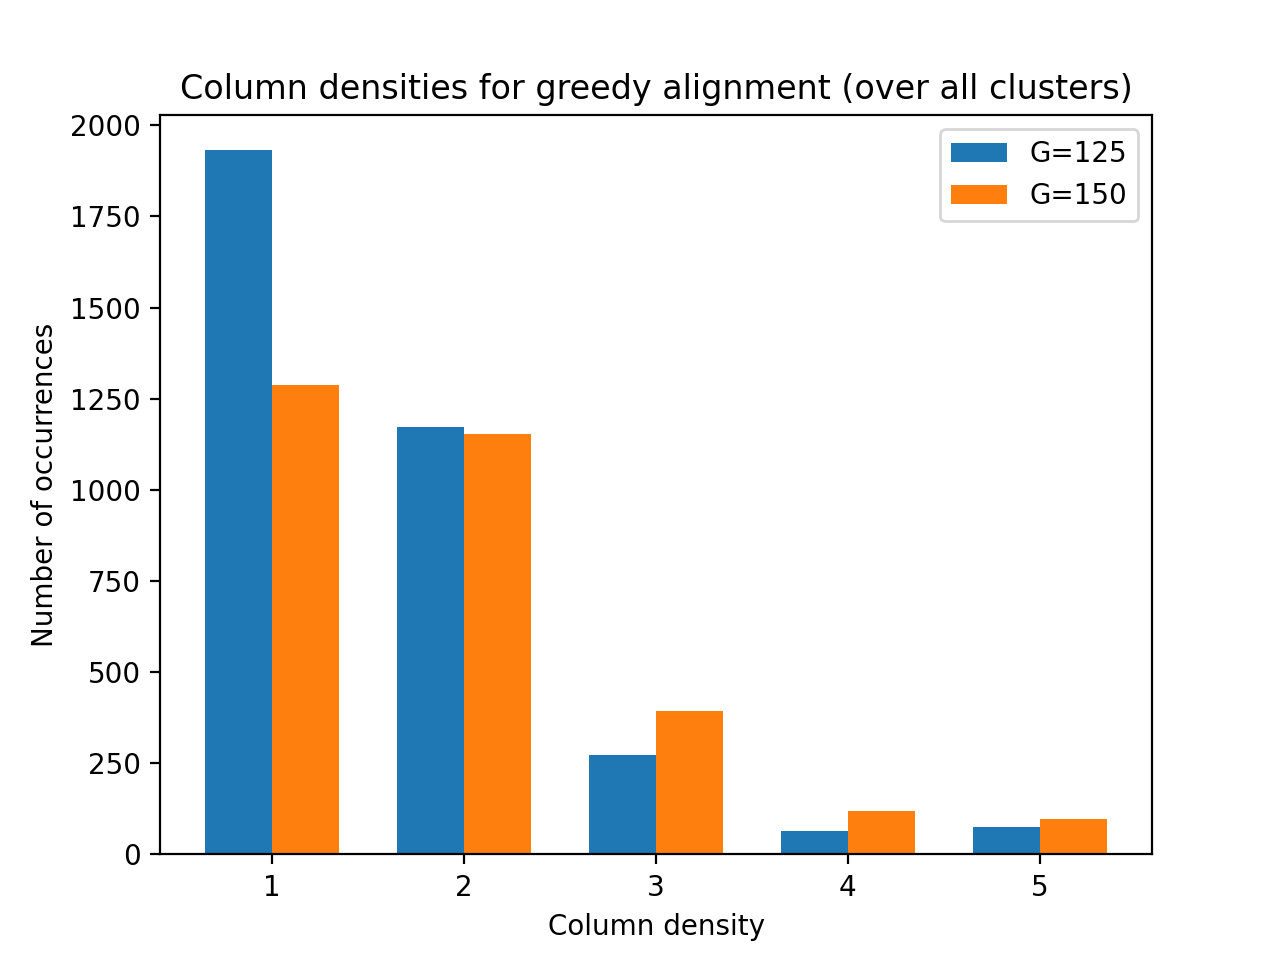
\includegraphics[width=3in]{img/prog125v150.png}
\caption{}
\end{subfigure}
\begin{subfigure}{0.5\textwidth}
\centering
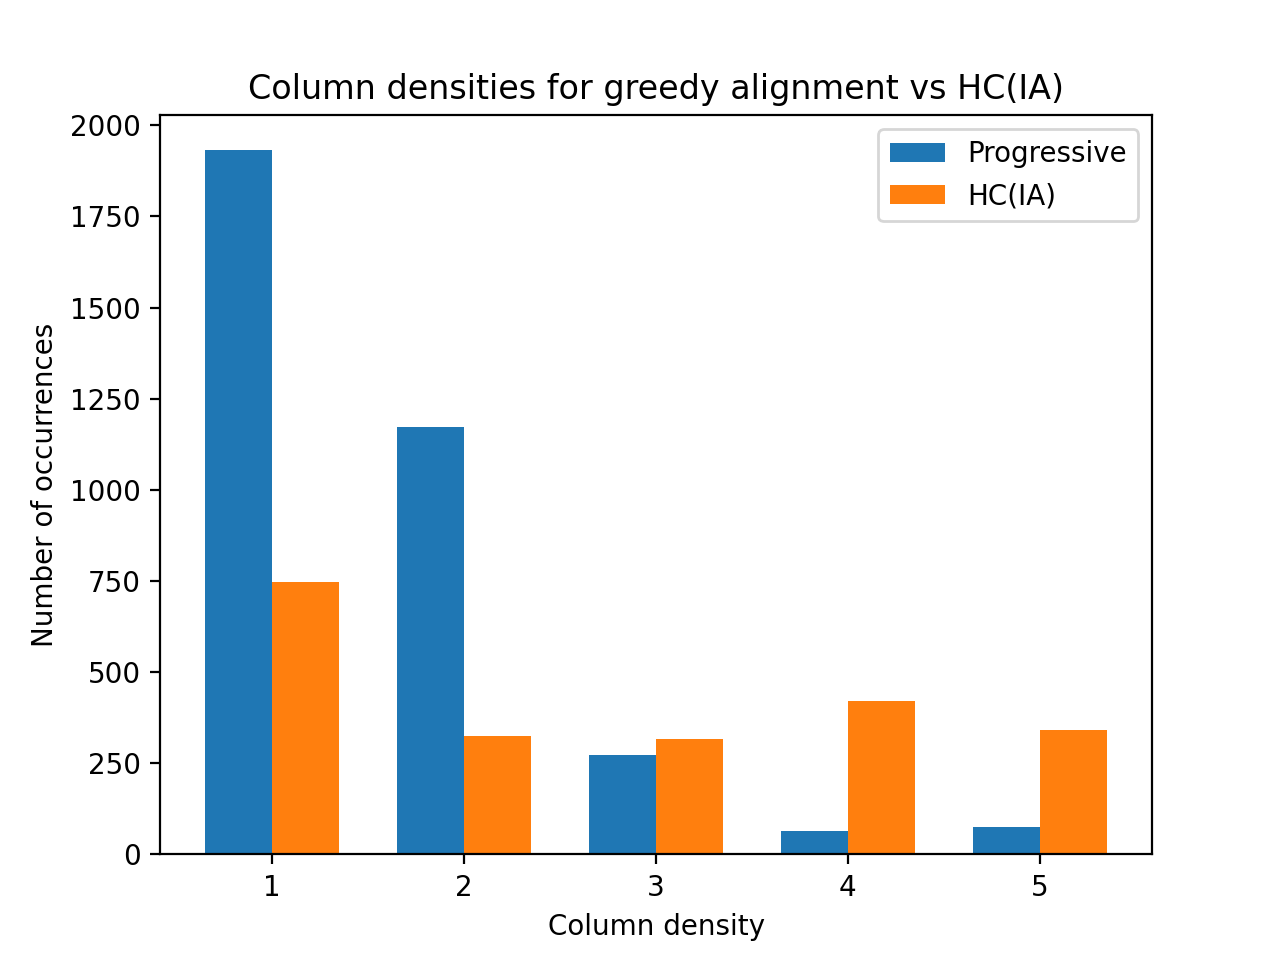
\includegraphics[width=3in]{img/prog125vhcia}
\subcaption{}
\end{subfigure}
\caption{
\label{fig:colcounts}
Merge into one graph.
}
\end{figure}




\newpage
\bibliographystyle{plainnat}
\bibliography{bib}

\end{document}
